% Compile: tectonic main.tex   (XeLaTeX engine; BibTeX run automatically)
\documentclass[11pt]{article}

\usepackage{fontspec}
\setmainfont{Libertinus Serif}
\setsansfont{Libertinus Sans}
\setmonofont[Scale=0.86]{DejaVu Sans Mono}

\usepackage{amsmath}
\usepackage[margin=1.15in]{geometry}
\usepackage{graphicx}
\usepackage{booktabs}
\usepackage{natbib}
\usepackage[small,labelfont=bf,margin=0.5cm]{caption}
\usepackage{microtype}
\usepackage{titlesec}
\usepackage{placeins}
\usepackage{xcolor}
\usepackage{hyperref}
\hypersetup{colorlinks=true, linkcolor={blue!45!black},
            citecolor={blue!45!black}, urlcolor={blue!45!black}}

\titleformat{\section}{\large\bfseries}{\thesection}{0.7em}{}
\titleformat{\subsection}{\normalsize\bfseries}{\thesubsection}{0.6em}{}
\setlength{\parskip}{0pt}
\bibliographystyle{apalike}

\newcommand{\project}[1]{\texttt{#1}}

\title{\LARGE The Small World of the Amarna Letters, Revisited:\\
\Large A Reproducible, Bias-Aware Network Analysis}
\author{Conor Reid}
\date{Working draft v0.2 --- August 2026\\
\small All numbers regenerate from \project{run\_all.sh}; seeds fixed.
Target venue: \emph{Journal of Historical Network Research}.}

\begin{document}
\maketitle

\begin{abstract}
\noindent The Amarna letters (c.~1360--1330 BC) are the oldest
well-preserved archive of interstate diplomacy, and the network analysis
of \citet{ClineCline2015} --- a hand-coded ``small world'' with
clustering ${\sim}49\times$ a random graph, brokered above all by
Rib-Hadda of Byblos --- has become the canonical quantitative reading of
the corpus. We rebuild the Amarna networks from the Oracc lemmatized
edition with fully reproducible code, hand-coding only what the digital
corpus lacks, and subject every headline claim to appropriate null models
and survival-bias corrections. Three results follow. (1)~The
correspondence network contains \emph{zero} triangles: the celebrated
small world lives entirely in the mention layer. Reconstructed at full
scale (244 persons; Cline \& Cline counted 246), that layer's clustering
(0.409~$\approx$ their 0.391) exceeds a fair bipartite configuration null
by a factor of ${\sim}1.6$ --- genuine structure, but far from the
``$48.75\times$'' figure produced by an Erdős--Rényi comparison.
(2)~Rib-Hadda's famous brokerage replicates exactly under Cline \&
Cline's construction and dissolves under bias correction: it depends on
splitting the pharaoh's identity across nodes and on his 60+-letter
dossier; volume-equalized, he falls to median rank~15 with zero bootstrap
probability of a top-three position, while Aziru of Amurru and the
Egyptian commissioner Yanḫamu emerge as the stable brokers.
(3)~Inferential models formalize the tier structure (ERGM: reciprocity
$+3.78$, tier anti-homophily $-2.21$, both $p<0.001$), and geography
behaves exactly as pre-registered: distance decays mention and conflict
ties but not correspondence with the court --- a result we report with
confidence only because an apparent counter-finding ($\rho=-0.50$ for
correspondence) dissolved under our own audit into gazetteer mismatches,
a tie-handling artifact, and political composition: an object lesson in
the paper's central argument, applied to ourselves. We release the actor
registry, edge lists, provenance joins (including a machine-readable
transcription of the petrographic determinations of
\citealp{Goren2004}), and all code.
\end{abstract}

\section{Introduction}

The 382 tablets found at Tell el-Amarna record the diplomatic
correspondence of the Egyptian court under Amenhotep~III and Akhenaten
with two tiers of partners: the ``Great Powers'' (Babylonia, Assyria,
Mittani, Hatti, Arzawa, Alashiya) and the vassal rulers of the Levant
\citep{Moran1992, Rainey2015, CohenWestbrook2000}. \citet{ClineCline2015}
introduced network analysis to this corpus, hand-coding actors and ties
in NodeXL, and reported three memorable findings: a clustering
coefficient of 0.391, ``nearly fifty times higher'' than a comparable
random network; the minor king Rib-Hadda of Byblos out-scoring both
pharaohs in betweenness centrality; and pharaohs dominating only two of
ten network clusters. \citet{Cline2025} brought this picture --- 246
named people, 464 connections --- to a broad audience.

These studies are exploratory: no null models, no uncertainty, no
correction for the archive's structure, and hand-coded data that cannot
be audited. The present study asks which of their findings survive
reproducible construction and appropriate inference --- and finds that
the answer is a precise decomposition rather than a verdict: each
headline claim is true under one specific set of constructional choices
and false under defensible alternatives. Identifying \emph{which} choice
drives \emph{which} result is, we argue, the useful contribution.

A second contribution is methodological framing, in the tradition of
archaeological network science's missing-data literature
\citep{Collar2015, BrughmansPeeples2023}. The archive is an ego-network
of Egypt, excavated in Egypt: every correspondence tie touches the court
by construction, and every mention survives because some letter to Egypt
carried it. Centrality measured on such an archive is \emph{salience to
Egypt}, not historical importance. Rather than treating this as a caveat,
we build it into the analysis: the correspondence layer is analyzed as
what it is (a star), the substantive questions are pushed to the mention
and conflict layers, and every centrality claim carries bootstrap rank
intervals and dossier-volume corrections.

\section{Data}

\paragraph{Corpus.} The Oracc \project{aemw/amarna} edition
\citep[catalogue timestamp 2024-07-05]{LauingerYoder2025} contains 379
catalogued tablets, of which 347 are letters and 305 carry lemmatized
transliteration (34,346 word tokens, 94.0\% lemmatized). The Great Powers
letters EA~1--44 and ${\sim}30$ fragments have catalogue metadata but no
digital text.

\paragraph{A correction to the record.} Contrary to the assumption
(reproduced in our own project plan from the Oracc pager configuration)
that the catalogue lacks structured sender/addressee fields, the raw
\project{catalogue.json} carries \project{ancient\_author} for 349 and
\project{recipient} for 348 of 379 entries --- including 42/44 of the
unlemmatized Great Powers letters. We therefore used the catalogue fields
as the primary source and demoted formula parsing to a validation
instrument.

\paragraph{Validation.} A parser extracting sender and addressee from
the stereotyped address formulae \citep[cf.][]{Mynarova2007} agrees with
the catalogue on 96.1\% (sender) and 96.5\% (addressee) of comparable
letters. All 18 disagreements were adjudicated against both English
editions \citep{Moran1992, Rainey2015}. Both editions confirm two
catalogue errors (EA~62 is addressed to the commissioner Paḫanate, not
pharaoh; EA~301 is from Šubandu, not Yapaḫu), as well as EA~7's recipient
(``Babylon'' corrected to the pharaoh Rainey restores as
[Napḫu]rureia). Twelve cases resolve for the catalogue with both editions
agreeing; three remain edition-contested and are graded \emph{disputed}.
Every verdict, with supporting quotations from both editions, ships in
the repository.

\paragraph{Entity resolution.} Actors are keyed on alias-canonicalized
folded names; the hand-curated registry (17 entries) records
Sumerographic readings (IR₃-Ḫebat = ʿAbdi-Ḫeba), orthographic systems
(Oracc ʿAḏiri = conventional Aziru), contested sign readings, and
pharaonic throne names, each with a justification; figure preparation
surfaced one residual split identity (Labʾayu keyed under both lemma and
catalogue spellings, similarly Milki-ilu), merged before the final run.
All named pharaohs collapse to a single PHARAOH node in the base
analysis; the per-letter identification is retained for sensitivity
splits.

\paragraph{Hand-coded supplements.} EA~1--44's mentioned persons were
coded from Moran's translations (44 letters; gods excluded, throne names
resolved to PHARAOH). A signed conflict layer (accusation/alliance) was
coded via a corpus-wide hostile-language sweep of Moran's translations
(40 letters, 63 edges: 59 accusations, 4 alliances), each edge carrying
its Moran quotation. The full set was then independently recoded from
Rainey's translations: cross-edition agreement is 93.5\% with Cohen's
$\kappa=0.86$, all divergences traceable to textual differences between
the editions rather than to the coding rules. This establishes
edition-robustness; since both passes share an annotator, an independent
human recoding remains the outstanding reliability step.

\paragraph{Geography and provenance.} Polities were georeferenced
against Pleiades (31/55 automated with hand-review flags; regions
without ancient fixed points remain unlocated by design). Four automated
matches proved to be classical homonyms at wildly wrong locations and
were corrected against the Pleiades bulk dump; \S\ref{sec:geography}
reports what that audit did to a headline number. The petrographic
provenance determinations of \citet{Goren2004} were transcribed to a
machine-readable table (292 tablets); where both sources speak, the
petrographic determination agrees with the catalogue's provenience 87\%
of the time, and the disagreements reproduce Goren et al.'s own
discoveries.

\section{Network construction}

Three layers, all built by code from the tables above:

\begin{enumerate}
\item \textbf{Correspondence} (directed, weighted): sender
$\rightarrow$ addressee per letter; 111 actors, 302 letters, 117
distinct dyads, every endpoint carrying a confidence grade.
\item \textbf{Mention co-occurrence} (undirected, weighted): the
persons appearing in each letter form a clique; 244 persons, 734 dyads.
The Great-Power letters enter via the Moran hand-coding.
\item \textbf{Conflict} (signed, directed; provisional): 63 accusation
($-$) and alliance ($+$) edges across 40 letters, with quotation-level
provenance.
\end{enumerate}

We additionally rebuild a \textbf{Cline-style graph} --- correspondence
edges plus sender$\rightarrow$mentioned stars --- because replication
requires the original's construction, not just its corpus.

\begin{figure}[tb]
\centering
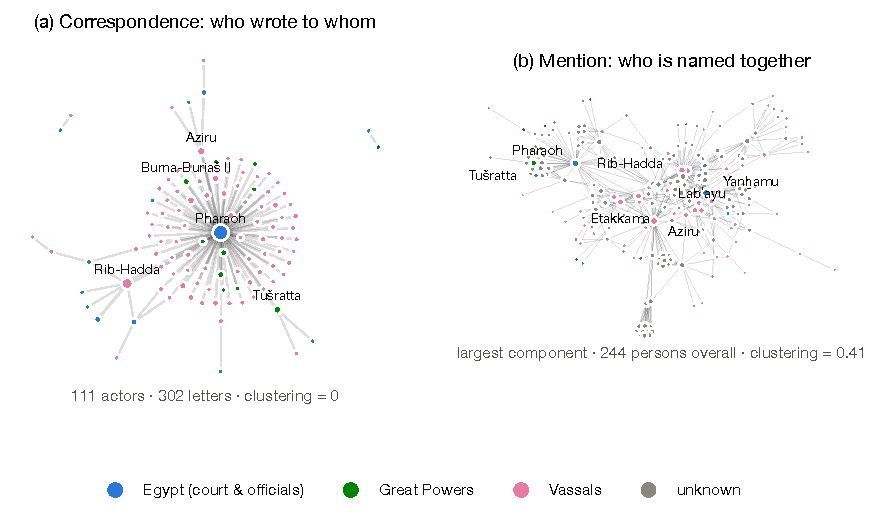
\includegraphics[width=\textwidth]{figures/fig1_two_layers.pdf}
\caption{The two layers of the Amarna network. (a)~The correspondence
layer is a star on the court: everyone writes to Egypt, and its global
clustering is exactly zero. (b)~The mention layer --- persons named
together in the same letter --- is where all triadic structure lives.
Node area scales with letter volume (a) and degree (b); layouts are
seeded Fruchterman--Reingold \citep{Csardi2006}.}
\label{fig:layers}
\end{figure}

\section{Methods}

Descriptives are never compared to an Erdős--Rényi baseline alone. The
correspondence and Cline-style graphs are tested against
degree-preserving rewiring; the clique-projected mention layer against a
\emph{bipartite} configuration null (shuffling person-to-letter
incidences while preserving letter sizes and person frequencies), since
clique projection manufactures triangles that edge-rewiring nulls do not
discount \citep{BrughmansPeeples2023}. Centrality claims carry
(a)~bootstrap-over-letters 95\% rank intervals (competition-ranked under
ties) and (b)~a dossier-equalization design in which every sender
contributes at most the median dossier size (2 letters) per replicate.
Inference: an ERGM on the binarized correspondence network
\citep{HunterHandcock2006, Handcock2008statnet}, with a Bayesian
replication \citep{CaimoFriel2011}; a latent-space cluster model on the
mention layer \citep{KrivitskyHandcock2008}; community detection by both
Louvain and Leiden \citep{Blondel2008, Traag2019}; and QAP/permutation
tests \citep{FreedmanLane1983} for the geography contrasts. All analyses
are seeded; \project{run\_all.sh} regenerates every number in this
paper.

\section{Results}

\subsection{The correspondence network has no small world to find}

Global and local clustering in the correspondence layer are exactly zero
in all three edge sets (all letters; high-confidence only; without the
Byblos dossier) --- below even the configuration null (95\% band
0.0015--0.0051). The layer is a star on Egypt
(Figure~\ref{fig:layers}a): vassals and kings wrote to the court, not to
each other (two vassal--vassal dyads exist in 302 letters). Whatever the
``small world of the Amarna letters'' is, it is not a property of who
wrote to whom.

\subsection{The small world is real, mention-borne, and
${\sim}1.6\times$ --- not $49\times$}

Rebuilt at full scale, the person-to-person mention network has 244
persons (Cline \& Cline: 246 people) and clustering 0.409 (theirs:
0.391) --- we take this convergence as evidence that we have
reconstructed their object. An Erdős--Rényi comparison of the kind
behind the ``$48.75\times$'' claim yields $16.5\times$ here. But against
the bipartite configuration null the observed 0.409 stands over a null
median of 0.253 (95\% band 0.235--0.271): significant --- the observed
value lies outside the null band in every variant, including without the
Byblos dossier (0.452 vs.\ 0.315) --- but a factor of ${\sim}1.6$
(Figure~\ref{fig:nulls}). The small world of the Amarna letters exists;
the astronomical multiplier was an artifact of the weakest available
null. The Cline-style star construction, by contrast, clusters at 0.034,
at or below its null --- confirming that triadic structure comes from
mentions connecting \emph{third parties}, not from anyone's
correspondence.

\begin{figure}[tb]
\centering
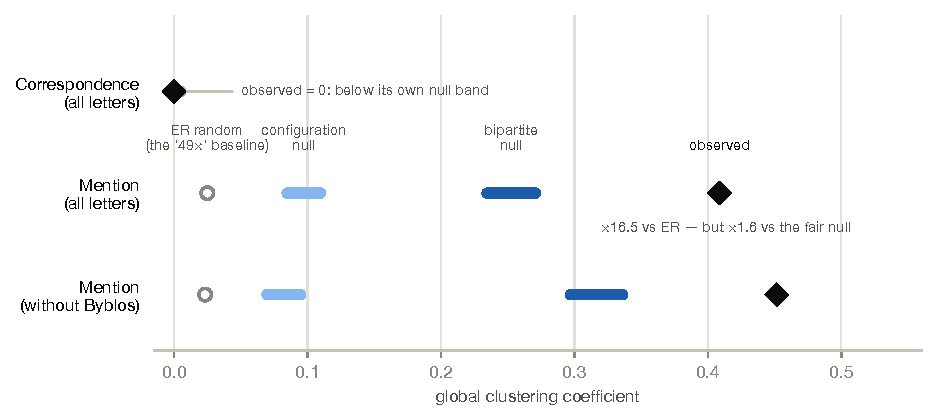
\includegraphics[width=\textwidth]{figures/fig2_nulls.pdf}
\caption{Observed clustering against three null models. The multiplier
one reports is a choice of null: against Erdős--Rényi the mention layer
is ${\sim}16\times$ ``random''; against a bipartite configuration null
that knows letters come in groups, ${\sim}1.6\times$. The correspondence
layer sits \emph{below} its own null band at exactly zero.}
\label{fig:nulls}
\end{figure}

\subsection{Rib-Hadda's brokerage, decomposed}

Cline \& Cline's flagship finding --- Rib-Hadda of Byblos out-brokering
the pharaohs --- replicates \emph{exactly} under their choices: in the
Cline-style graph with pharaohs split by identification, Rib-Hadda's
betweenness exceeds Amenhotep~III's and Amenhotep~IV's. But the residual
unidentified pharaoh --- most letters address only ``the king'' ---
holds roughly five times Rib-Hadda's score. The finding is an artifact
of dividing one actor's identity across nodes under uncertainty. From
there the correction proceeds stepwise (Figure~\ref{fig:ribhadda}):
collapse the pharaohs and Rib-Hadda is second; move to the
person-to-person layer and he is ${\sim}$7th (bootstrap median 7, 95\%
interval 4--12); equalize dossier volume and he is 15th with
$P(\text{top }3)=0.00$. His 63-letter dossier buys eigenvector
attachment to the hub, and nothing else.

The stable brokers, in every construction and correction, are
\textbf{Aziru of Amurru} (rank~1 with $P(\text{top }3)=0.94$--$0.98$
across designs) --- the defector who bridged Egypt's orbit and Hatti's,
and simultaneously the most-accused actor in the conflict layer
(Figure~\ref{fig:conflict}) --- and, once volume is corrected,
\textbf{Yanḫamu}, the Egyptian commissioner ($P(\text{top }3)=0.66$),
vindicating the hypothesis that pharaoh's officials, not the loudest
vassal, carried the network. Rib-Hadda's fame is a fact about his
archive, not his position.

\begin{figure}[tb]
\centering
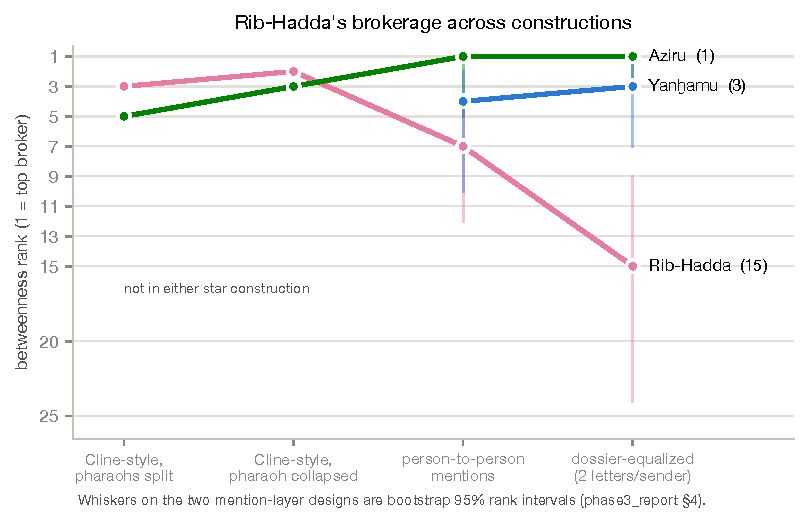
\includegraphics[width=0.85\textwidth]{figures/fig3_ribhadda.pdf}
\caption{Betweenness rank of three actors across four constructions,
from Cline \& Cline's split-pharaoh graph (left) to the
dossier-equalized mention layer (right). Rib-Hadda's celebrated
brokerage exists only in the star constructions; Aziru holds rank~1 in
every corrected design, and the commissioner Yanḫamu --- invisible in
either star construction --- rises once volume is equalized.}
\label{fig:ribhadda}
\end{figure}

\begin{figure}[tb]
\centering
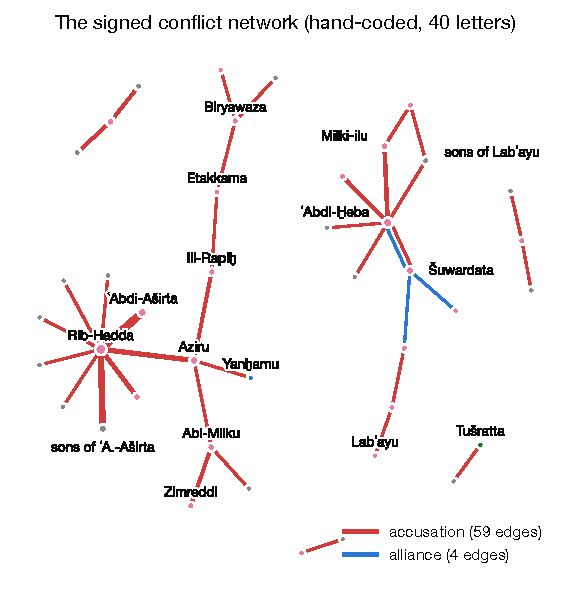
\includegraphics[width=0.9\textwidth]{figures/fig6_conflict.pdf}
\caption{The signed conflict network, hand-coded from hostile and allied
language (edges drawn undirected; both an accusation and an alliance
connect Šuwardata and ʿAbdi-Ḫeba, EA~366). The regional theatres ---
Amurru (left), Damascus--Qadesh (center), Shechem--Jerusalem (right) ---
are invisible in the correspondence layer.}
\label{fig:conflict}
\end{figure}

\subsection{The diplomatic system as coefficients}

The ERGM formalizes the two-tier reading \citep[cf.][]{Liverani2001,
Podany2010}: reciprocity is strong and significant
($\text{mutual}=+3.78\pm0.80$), concentrated at the Great-Power tier
(17\% of Egypt$\leftrightarrow$Great-Power dyads reciprocated vs.\ 4\%
of Egypt$\leftrightarrow$vassal, the latter being Egyptian file copies),
and tier homophily is strongly \emph{negative}
($\text{nodematch}=-2.21\pm0.64$): Amarna correspondence is cross-tier
by construction --- the brotherhood of kings and the servitude of
vassals both materialize as letters to Egypt, not within-tier
correspondence (Table~\ref{tab:ergm}). The Bayesian replication agrees
(mutual 95\% credible interval $[2.3, 6.2]$; nodematch $[-4.0, -0.8]$).
The latent-space model finds clusters that do not recover the tiers:
mention-layer communities (modularity ${\approx}0.56$) are political
theatres --- the Amurru crisis, the Damascus--Qadesh axis, the
Shechem--Jerusalem conflict, the Tyre--Sidon feud --- not diplomatic
ranks.

\begin{table}[tb]
\centering\small
\caption{ERGM on the binarized correspondence network (MCMLE; GOF
adequate on all model statistics, MC $p\ge0.94$). The Bayesian
replication (Bergm, 30k iterations) gives concordant posteriors.}
\label{tab:ergm}
\begin{tabular}{lrrr}
\toprule
term & est. & s.e. & $p$ \\
\midrule
edges & $-2.58$ & 0.68 & 0.0002 \\
mutual (reciprocity) & $+3.78$ & 0.80 & $<0.0001$ \\
receiver: Great Power & $-4.20$ & 0.77 & $<0.0001$ \\
receiver: vassal & $-4.07$ & 0.53 & $<0.0001$ \\
sender: Great Power & $+0.12$ & 0.73 & 0.86 \\
sender: vassal & $+0.11$ & 0.68 & 0.87 \\
tier homophily (nodematch) & $-2.21$ & 0.64 & 0.0006 \\
\bottomrule
\end{tabular}
\end{table}

\subsection{Geography: the pre-registered contrast, recovered by audit}
\label{sec:geography}

Distance decays ties in the mention layer (point-biserial $r=-0.147$,
QAP $p<0.001$): neighbors name neighbors. The conflict layer agrees
($r=-0.298$, QAP $p=0.001$, $n=14$ located actors). We had predicted
\emph{no} distance effect in the correspondence layer --- all vassals
write to distant Egypt regardless --- and an earlier draft reported that
prediction overturned ($\rho=-0.50$, $p=0.002$). Auditing that finding
dissolved it, in three layers that are worth recounting because they
enact the paper's thesis. First, six of 39 data points were gazetteer
phantoms (Figure~\ref{fig:audit}): four actors coded to a ``Syria''
\emph{region} whose Pleiades match lies in the Ionian Sea, Pihilu
matched to Macedonian Pella, Irqata to an Anatolian Arca --- all
far-with-few-letters, exactly the shape that manufactures decay (Tyre
was likewise mislocated to a homonymous Hellenistic estate in Jordan).
Second, with 14 of 35 vassals tied at one letter, Spearman without
tie-averaged ranks let input row order leak into the statistic;
correcting both leaves $\rho=-0.32$ ($p=0.07$). Third, the residual
trend is compositional: it concentrates in polities with political
reasons to write little --- Hatti-aligned Qadesh and Sidon (EA~174--176,
148--149) and quasi-independent Ugarit --- without which $\rho=-0.18$
($p=0.32$); a leave-one-polity-out jackknife retains nominal
significance in only 7 of 24 deletions. A partialled design against
hand-coded covariates --- distance to the nearest Egyptian
administrative center (Gaza, Joppa, Beth-Shean, Kumidi, Ṣumur;
Figure~\ref{fig:map}; cf.\ \citealp{Morris2005}), coastal access, Hatti
alignment --- finds no predictor of epistolary volume, court distance
included (partial $r=-0.26$, $p=0.17$). The sign stays negative in every
variant, so a weak true decay is not excluded; but the defensible
statement is the pre-registered one: geography structures whom the
letters \emph{talk about}, not who talks to Egypt.

\begin{figure}[tb]
\centering
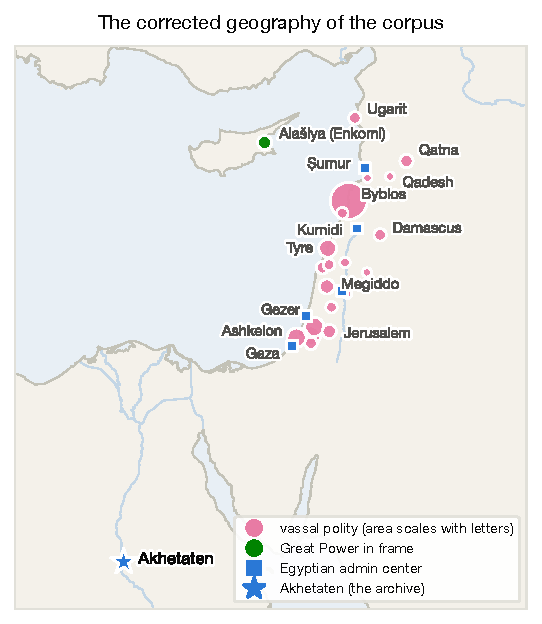
\includegraphics[width=0.62\textwidth]{figures/fig4_map.pdf}
\caption{The corrected geography of the corpus: located vassal polities
(area scales with letters to pharaoh), the five Egyptian
garrison/commissioner seats used as the administrative-density
covariate, and Akhetaten. Region-states without fixed points (Amurru,
Mittani, ``Syria'') are excluded rather than imputed.}
\label{fig:map}
\end{figure}

\begin{figure}[tb]
\centering
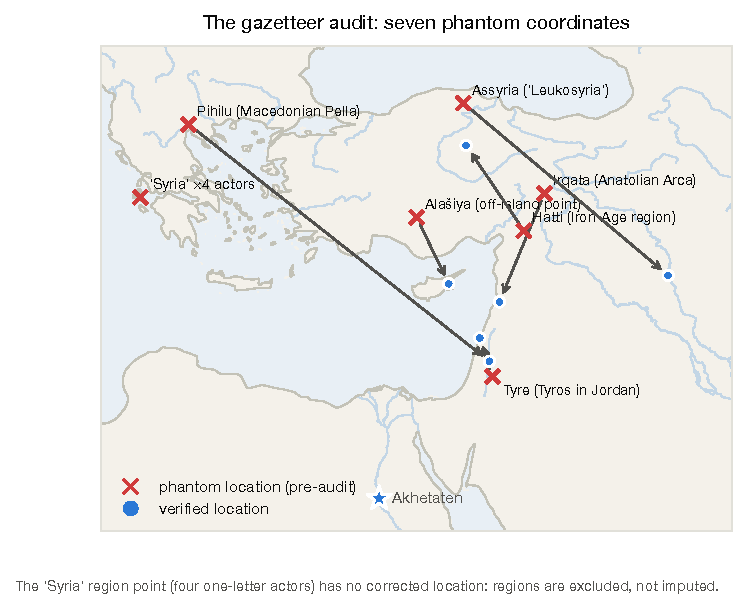
\includegraphics[width=\textwidth]{figures/fig5_audit.pdf}
\caption{The gazetteer audit. Seven ``phantom'' coordinates produced by
homonym mismatches against a classical gazetteer (crosses), with their
verified locations (dots). All seven pushed in the decay direction ---
far-with-few-letters --- and together with a rank-tie artifact they
manufactured the apparent correspondence distance decay
(\S\ref{sec:geography}).}
\label{fig:audit}
\end{figure}

\FloatBarrier
\section{Discussion}

The revision this study proposes is not that Cline \& Cline were wrong
but that each of their results is the output of an unstated
constructional switch. Split the pharaoh's identity and Rib-Hadda
out-brokers kings; collapse it and he does not. Compare against an
Erdős--Rényi graph and the archive is a $49\times$ marvel; compare
against a null that knows letters come in groups and it is a $1.6\times$
society. Count a man's own dossier and he is central; ask what remains
when every voice speaks at equal volume and the brokers are the defector
Amurru dynast and pharaoh's own commissioner. None of these switches is
illegitimate --- but they must be visible, and their consequences
measured, before centrality in a survival-biased ego-archive is read as
ancient history. Our own distance-decay episode
(\S\ref{sec:geography}) shows the same failure mode operating inside a
reproducible pipeline, and the same remedy: the error survived exactly
as long as the underlying data points went unexamined.

What survives every correction is historically satisfying: a two-tier
system statistically legible in one coefficient ($+$ reciprocity above,
$-$ homophily across), inter-vassal politics organized in regional
conflict theatres invisible to the correspondence graph, brokerage
lodged in exactly the two figures --- Aziru, Yanḫamu --- whose careers
the letters narrate as boundary-crossing, and a mention society whose
modest but real small-world excess reflects genuine third-party
political entanglement. The archive measures salience to Egypt; measured
carefully, that salience still has structure worth explaining.

\section{Limitations}

The conflict layer is corpus-wide and edition-robust (cross-edition
$\kappa=0.86$) but single-annotator; an independent human recoding
remains desirable. EA~1--44 mentions were hand-coded from translation
rather than lemmata (a documented source seam that will close when Oracc
releases the Great Powers letters). Senders whose polity the catalogue
string does not state default to the vassal tier (14 minor
correspondents of 1--3 letters each); Ugarit's rulers are likewise coded
vassal though the kingdom's standing was closer to
client-of-both-courts. At these actors' letter volumes neither choice
can move the tier coefficients, but both are choices, not facts.
Chronology is coarse by design: a two-phase sensitivity split reproduces
the small-world excess within each era and keeps brokerage with the
Amurru dynasty in both --- ʿAbdi-Aširta early, Aziru late. Geographic
coverage reaches 64\% of letters at both endpoints; the excluded
region-states include Amurru, so the compositional analysis of
\S\ref{sec:geography} cannot see the system's most consequential
defector.

\section{Data and code availability}

All code (MIT), derived tables (CC-BY), figures, and this draft:
\url{https://git.sr.ht/~calgacus/ussira-pitati}. Oracc corpus text is
CC-BY-SA \citep{LauingerYoder2025} and is not redistributed; Moran
(1992) and Goren et al.\ (2004) are quoted within scholarly fair use. A
Zenodo deposit with DOI accompanies submission.

\bibliography{references}

\end{document}
